\documentclass[english]{ifacconf}
\usepackage[utf8]{inputenc}
\usepackage{array}
\usepackage{float}
\usepackage{amsmath}
\usepackage{amssymb}
\usepackage{graphicx}
\usepackage{natbib}
%\usepackage[unicode=true]{hyperref}

\begin{document}
\begin{frontmatter}
	
\title{Shared Decision-Making and Adaptive Output-Feedback Control for UAV Anomaly Mitigation}

%\thanks[footnoteinfo]{Sponsor and financial support acknowledgment
%goes here. Paper titles should be written in uppercase and lowercase
%letters, not all uppercase.}

\author[First]{Benjamin T. Thomsen} 
\author[First]{Anuradha M. Annaswamy} 

\address[First]{Massachusetts Institute of Technology, 
   Cambridge, MA 02139\\email: [thomsen, aanna]@mit.edu}

\begin{abstract}
This paper outlines a shared decision-making and control framework to recover control performance following anomalous changes in plant dynamics. Autonomous model-based controllers, including model reference adaptive control, rely on accurate modeling of dynamical systems and make assumptions about the relative time constants of unmodeled dynamics. Online changes to these unmodeled dynamics may cause degraded command tracking performance and a loss of stability. We introduce a shared control architecture in which a human supervisor (operator) may make suitable changes to the control model of the system following anomalous plant behavior to allow for continued autonomous adaptive control without transferring control responsibilities to the human operator.
\end{abstract}
\begin{keyword}
Five to ten keywords, preferably chosen from the IFAC keyword list.
\end{keyword}

\end{frontmatter}

\section{Introduction}
%Adaptive control and modeling assumptions.
Model-based feedback control techniques, where control design is carried out based on \textit{a priori} knowledge of system dynamics, have become ubiquitous in industries such as aerospace, due to their ability to specify characteristics of the closed-loop system dynamics, ensure stability, and provide optimality over a range of operating conditions. The field of adaptive control (MRAC) addresses a limitation of control based on models of plant dynamics, namely that the parameters used to model dynamical systems will always have a degree of uncertainty in them. Model reference adaptive control, as described by \cite{narendra2012stable}, accommodates these parametric uncertainties through online tuning of control parameters to ensure specified closed-loop dynamics are realized. Recent advances in MRAC have included the development of closed-loop reference models (CRMs) by \cite{gibson2013adaptive}, which greatly improves transient performance during online learning. While adaptive control is able to guarantee stability and tracking convergence in the presence of parametric uncertainties, other aspects of the system -- such as its order -- are assumed to be known \textit{a priori} for control design. 
%In practice, dynamical behavior is excluded from the control model for simplicity and ease of analysis if it sufficiently fast relative to the closed-loop system bandwidth.

%Human pilots and operators, and their struggles with unfamiliar, off-nominal dynamics. %Remote human pilots and further difficulties
Human operators of dynamical systems also develop mental models of the dynamics of the systems which they are controlling, often over long periods of active learning. Human pilots have been studied extensively to examine their learning processes and ability to adapt their control strategies to unfamiliar situations. When unexpected changes occur during operation, however, it is often difficult for human operators to learn the new dynamics in the time period necessary to avoid loss of control. Numerous aircraft accidents have involved pilot error following a transition from autonomous to manual control. Studies of human pilot behavior have repeatedly demonstrated how pilots operating in stressful situations controlling unfamiliar dynamics resort to applying high control gains, which can lead to a loss of stability margins and exceedence of the aircraft flight envelope. Issues with manual control of dynamical systems are exacerbated when the human operator is physically separated from the dynamics of the system, as is the case with remotely piloted vehicles (RPV). The additional complexities involved with remote operation include a lack of physical sensing of the dynamics through proprioceptive and somatosensory pathways, time delays between the vehicle and operator for both sensing and actuation, and difficulty ascertaining the open-loop dynamical response between control input and plant output. 

%HALE VFA.
Solar-electric high altitude long endurance (HALE) aircraft concepts have recently received heavy attention as key enabling technologies has advanced to allow for feasible months-long unmanned operation of these aircraft. These concepts, such as the NASA/AeroVironment Helios, sacrifice structural rigidity to decrease vehicle mass, and are thus classified as very flexible aircraft (VFA). For additional mass reductions, it may be desirable to use small actuators which introduce slow dynamics which must be accounted for in control design. The benefits derived from weight savings in HALE VFA platforms -- and the fact that they are unmanned -- may lead to designs with more modeling uncertainties and potential for online variations in dynamics.

\section{Problem Statement}\label{sec:problem}
%Control of plant with unknown/uncertain parameters. 
We consider control design for a linear multi-input multi-output (MIMO) plant model of the form
\begin{equation}
\begin{gathered}
\dot x_p = (A_p + B_p \Theta_p^T) x_p + B_p \Lambda_p u_p \\
y_p = C_p x_p, \qquad z_p = C_{pz} x_p \label{eq:plant_dynamics}
\end{gathered}
\end{equation}
where uncertain dynamics lead to the introduction of unknown $\Theta_p$ and $\Lambda_p$ in the plant model, $y_p$ are measurement outputs, and $z_p$ are regulated (tracking) outputs. It is assumed that the plant has uniform relative degree unity (matrix $CB$ has full rank), and in addition to the dynamics (\ref{eq:plant_dynamics}), the vehicle's actuators are modeled by the first-order dynamics
\begin{equation}
	\dot{u}_p + (D_1 + \Theta_1^T) u_p = D_1 u \label{eq:first_order_act}
\end{equation}
where $D_1$ is a diagonal matrix representing nominal actuator parameters and $\Theta_1$ models uncertainty in the actuator dynamics. Model reference adaptive control (MRAC) with output feedback and closed-loop reference models, as described by \cite{qu2016adaptive}, can achieve asymptotic tracking and guarantee stability for this control problem. 

The scenario motivating this paper is a sudden change in actuator dynamics during operation from (\ref{eq:first_order_act}) to the second-order model
\begin{equation}
	\ddot{u}_p + (D_2 + \Theta_2^T) \dot{u}_p + (D_1 + \Theta_1^T) u_p = D_1 u \label{eq:second_order_act}
\end{equation}
This introduction of unmodeled dynamics means that the assumptions used for control design no longer hold, and the autonomous controller may lose stability and command tracking ability. 

In addition to the autonomous controller which generates control input $u$ in (\ref{eq:first_order_act}) and (\ref{eq:second_order_act}), there is a human supervisor tasked with the high-level operation of the plant (\ref{eq:plant_dynamics}), including mission and task planning (commanding its mode of operation) and monitoring to ensure safe and anomaly-free operation. In this paper, we consider \textit{remote} human operators who cannot sense the vehicle state and dynamics directly through vestibular or somatosensory pathways. The human supervisor may be responsible for the supervision of multiple plant instances, as illustrated in Fig. \ref{fig:uav_supervisor} for the case of HALE VFA platforms. The remote human supervisor has information on vehicle measurement output, state, tracking performance, and health (via visual, tactile/haptic, and auditory interfaces), and is able to actuate the vehicle through the same pathways as the autonomous controller -- $u$ in (\ref{eq:first_order_act}) and (\ref{eq:second_order_act}) -- via remote controls. Both the sensing and actuation by the remote human supervisor include time delays $\tau_s, \tau_a > 0$.

The problem we investigate is whether autonomous control methodologies can be used in conjunction with a remote human supervisor to successfully mitigate the anomalous dynamics (\ref{eq:second_order_act}) and restore tracking performance in the presence of uncertainty. We refer to this class of anomaly response as a shared control response.

\begin{figure}[htbp]
	\centering
	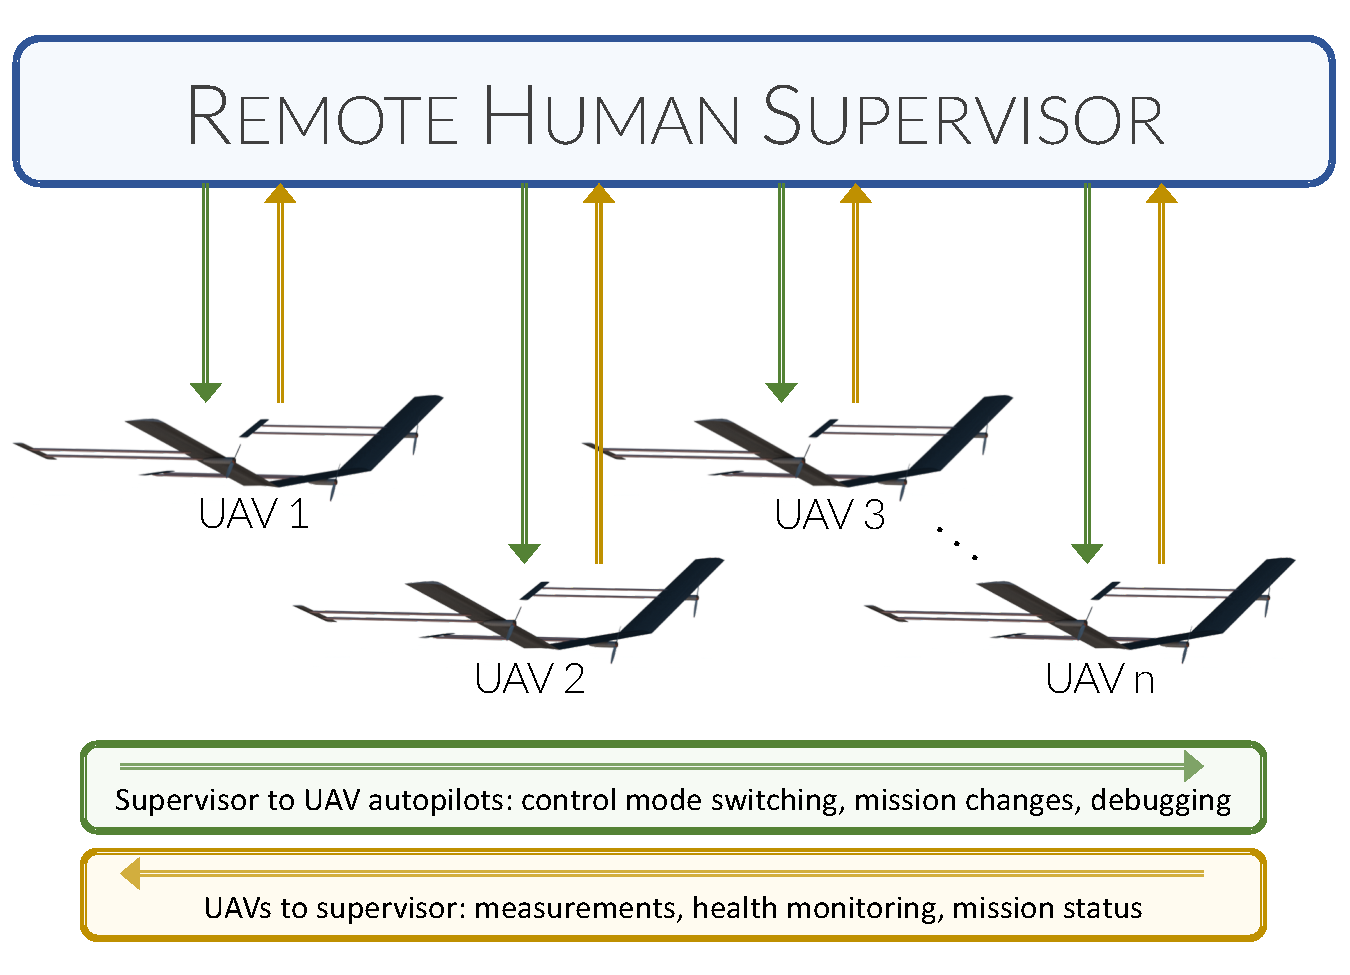
\includegraphics[width=0.95\columnwidth]{../fig/uav_supervisor.pdf}
	\caption{Supervisory operation of a fleet of HALE UAVs}
	\label{fig:uav_supervisor}
\end{figure}

%Recovery of closed-loop autonomous control performance following the introduction of severe anomalous dynamics to the plant. 

%Human supervisor is present (remotely), but should not be given control responsibilities following anomaly.

\section{Shared Control}\label{sec:shared_ctrl}
%Overview of shared control architecture. What is assumed?
We introduce a shared decision-making and control framework which we posit will enable the safe operation of HALE UAVs subject to both parametric uncertainties and the sudden introduction of unmodeled dynamics as described in the preceding section. This shared control framework is based on a combination of actions by UAV autopilots and remote human supervisors/operators, based on the framework for shared control proposed by \cite{thomsen2018shared}. MRAC autopilots and complementary higher-level guidance functions allow for continuous autonomous operation of the UAVs under nominal conditions. Remote human operators are constantly monitoring the performance of the vehicles and are trained and able to remotely pilot the vehicle in case of autopilot failure. The remote piloting of the vehicles, however, is a daunting task due to potential communication delays and a weakened understanding of the vehicle dynamics and state due to the remote (not onboard) nature. Our shared control framework involves the use of the remote human operator to diagnose and correct for the dynamical anomaly without taking over manual control of the vehicle. We will demonstrate how suitable adaptive autopilot functionalities allow for this possibility.

%Division of responsibilities.

\subsection{Adaptive Output-Feedback Control}\label{subsec:sc_adaptive}
%An autonomous controller is designed  to track commands for vertical acceleration of the VFA while regulating the dihedral angle. The control goal for ``nominal'' operation is to design linear controllers which are able to:
%\begin{enumerate}
%	\item Accommodate errors and uncertainty in the nonlinear model which is trimmed and linearized for control design, which we model as state-dependent and input-dependent parametric uncertainties in the linearized system
%	\item Account for slow first-order linear actuators dynamics with uncertainty in the DC gain and bandwidth (also captured as parametric uncertainties in the linearized system)
%\end{enumerate}
%using measurements of the pitch rate, dihedral angle, and vertical acceleration only. To accomplish these goals, we develop the ``nominal'' controller with the following components.
%\begin{enumerate}
%	\item A baseline control design using the linear quadratic regulator method with feedback on integrated tracking error (LQR-PI)
%	\item An adaptive output-feedback augmentation designed for the MIMO relative degree two dynamics which arise from including actuator dynamics, to handle the parametric uncertainties introduced
%\end{enumerate}
%
%The adaptive controller uses a \textit{closed-loop reference model} (CRM) for model following, which functions simultaneously as an observer for the baseline LQR-PI control, as described in \cite{lavretsky2015robust}.
An autonomous controller is designed  to track commands for vertical acceleration of the VFA while regulating the dihedral angle. To achieve the control goals stated in Section \ref{sec:problem} (namely the state-dependent and input-dependent parametric uncertainties in the plant as well as the actuator dynamics with uncertain parameters), we develop the ``nominal'' controller with the following components.
\begin{enumerate}
	\item A baseline control design using the robust servomechanism linear quadratic regulator method (RSLQR)
	\item An adaptive output-feedback augmentation designed for the MIMO relative degree two dynamics which arise from including actuator dynamics, to handle the parametric uncertainties introduced
\end{enumerate}
The shared control framework involves separate MRAC designs for the plant (\ref{eq:plant_dynamics}) in combination with actuator dynamics (\ref{eq:first_order_act}) and (\ref{eq:second_order_act}). The control design for (\ref{eq:plant_dynamics}) and (\ref{eq:first_order_act}) is the ``nominal'' control design, and excluding exceptional failures, this is the controller in use by the UAV autopilot. The control design for (\ref{eq:plant_dynamics}) and (\ref{eq:second_order_act}) is a predefined ``recovery'' controller, whose use case will be defined more fully in Section \ref{subsec:sc_human}.

Both of these control designs use an augmented linear plant formulation, where the plant (\ref{eq:plant_dynamics}) is extended with the linear actuator dynamics -- either (\ref{eq:first_order_act}) or (\ref{eq:second_order_act}) -- as well as integrated tracking errors 
\begin{equation}
	e_z^{\mathcal{I}}(t) = \int_0^{t} \big( z_p(\tau) - z_{cmd}(\tau)\big) d\tau
\end{equation}
in order to to use the RSLQR control design.

The augmented plant model with $x = \begin{bmatrix} x_p^T & x_{act}^T & (e_z^{\mathcal{I}})^T\end{bmatrix}^T$ can written compactly as
\begin{equation}
\begin{array}{c}
\dot{x}= \left(A+B_{1}\Psi_{1}^{T}+B_{r}\Psi_{r}^{T}\right) x+B_{r}\Lambda u+B_{z}z_{cmd}\\
y=Cx,\qquad z=C_{z}x
\end{array} \label{eq:augmented_plant}
\end{equation}
where $x\in\mathbb{R}^{n}$, $u\in\mathbb{R}^{m}$, $y\in\mathbb{R}^{p}$ are redefined states, inputs and outputs, respectively. A full justification for this form of the plant can be found in \cite{qu2016phd, qu2016adaptive}. This plant contains unknown matrices $\Psi_1$, $\Psi_r$, and $\Lambda$, which hold the state-dependent plant uncertainties, state-dependent actuator dependencies, and actuator effectiveness, respectively. The exact forms of $B_r$ and $\Psi_r$ depend on whether the actuators are first-order (\ref{eq:first_order_act}) or second-order (\ref{eq:second_order_act}), and the subscript $r$ indicates the relative degree of the augmented plant.

For control design, closed-loop reference models are designed as
\begin{equation}
\dot{x}_m = A_m x_m + B_z z_{cmd} + L e_y + \mathcal{F}_r(t), \quad y_m = C x_m
\end{equation}
where $e_y = y - y_m$, $A_m = A - B_r K^T$ with $K\in\mathbb{R}^{n\times m}$ is a nominal Luenberger-like feedback gain designed for the system without uncertainty, using the robust servomechanism linear quadratic regulator (RSLQR) design method (see \cite{lavretsky2013robust}). $\mathcal{F}_r(t)$ is a function used when $r \geq 2$ to recover stability properties in the presence of uncertainty. For sake of brevity, readers are referred to \cite{qu2016phd} and \cite{qu2016adaptive} for full derivations of the adaptive controllers used in this article. In what follows, we will summarize the design for the ``nominal'' controller and for the ``recovery'' controller, and assume the augmented plant model (\ref{eq:augmented_plant}) is square (i.e. $m = p$) for simplicity.
 
%This augmented model is defined by nominal state, input, and output matrices
%\begin{equation}  \small
%\begin{aligned}
%	A &= \begin{bmatrix}
%		\begin{matrix} A_p \\ 0 \\ C_{pz}	
%		\end{matrix}
%		& \begin{bmatrix}
%		\begin{matrix} B_p & 0 \end{matrix} \\
%		A_{act} \\
%		0 \end{bmatrix}
%		 & \begin{matrix} 0 \\ 0 \\ 0 \end{matrix}
%	\end{bmatrix}\\
%	B_1 &=
%	\begin{bmatrix}
%		B_p \\ 0 \\ 0
%	\end{bmatrix}, \quad B_r = 
%	\begin{bmatrix}
%		0\\ B_{act} \\ 0
%	\end{bmatrix}, \quad B_z = \begin{bmatrix}
%		0 \\ 0 \\ -I
%	\end{bmatrix} \\
%	C &= \begin{bmatrix}
%	C_{p} & 0 & 0\\
%	0 & 0 & I
%	\end{bmatrix}, \quad C_z = \begin{bmatrix}
%	C_{pz} & 0 & 0\end{bmatrix}
%\end{aligned}
%\end{equation}
%as well as uncertainty matrices given by
%\begin{equation} \small
%\Psi_{1}=\begin{bmatrix}
%\Theta_{p} \\ 0 \\ 0 \end{bmatrix}, \quad
%\Psi_{r}= -\begin{bmatrix} 0 \\ \begin{bmatrix}\Theta_1^{T} & \cdots & \Theta_k^{T} \end{bmatrix}^T \\ 0\end{bmatrix} (D_1)^{-1} 
%\end{equation}

\subsubsection{Nominal Adaptive Control Design}
%Relative degree two MIMO adaptive control.
% need a11, a10, B_1^a, Cbar, S, Rinv, epsilon, L, two tuner laws, u, F
The control design for the plant with first-order actuator dynamics will be summarized by giving definitions for feedback gain $L$, function $\mathcal{F}_2(t)$, control law $u$, and parameter adaptation. First, we will use $B_2$ to denote $B_r$ from (\ref{eq:augmented_plant}) for this relative degree two plant. The feedback matrix $L$ is designed by defining relative degree 1 input path
\begin{equation}
B_1^a = \alpha_0 B_2 + \alpha_1 A B_2 \label{eq:rd2-b1a}
\end{equation}
where $\alpha_i > 0$ are free design parameters. We then define
\begin{align}
S &= (C B_1^a)^T \label{eq:S}\\	\overline{C} & = S C\\ R^{-1} &= (\overline{C} B_1^a)^{-1} \big[ \overline{C} A B_1^a + (\overline{C} A B_1^a)^T\big] (\overline{C} B_1^a)^{-1} + \epsilon I \\ L & = B_1^a R^{-1} S \label{eq:L}
\end{align}
where $\epsilon > 0$ \cite[Eq. 30]{qu2015adaptive} is chosen to guarantee stability of the adaptive system. 

The function $\mathcal{F}_2(t)$ makes use of scaled error signal
\begin{equation}
	e_{sy}(t) = R^{-1} S e_y(t) \label{eq:esy}
\end{equation}
and a filtered version of this signal, $\overline{e}_{sy}(t)$, given in the form of a differential equation as
\begin{equation}
(\alpha_0 + \alpha_1 \frac{d}{dt}) \big\{ \overline{e}_{sy}(t) \big\} = \alpha_1 e_{sy}(t) \label{eq:e_sy_bar}
\end{equation}
It is worth noting that this can be represented in the frequency domain as
\begin{equation*}
	\overline{E}_{sy}(s) = \frac{\alpha_1}{\alpha_1 s + \alpha_0} E_{sy}(s)
\end{equation*}

The function is then defined as
\begin{equation}
\mathcal{F}_2(t) = B_2 (\alpha_0 + \alpha_1 \frac{d}{dt})\big\{ \hat{\Psi}_m^T (t) \bar{e}_{sy}(t) \big\}
\end{equation}
where $\hat{\Psi}_m(t)$ is a matrix of adaptive parameters, defined more fully in \cite{qu2016adaptive}. Similar to (\ref{eq:e_sy_bar}), we define filtered reference model state, $\overline{x}_m(t)$, with the differential equation
\begin{equation}
(\alpha_0 + \alpha_1 \frac{d}{dt}) \big\{ \overline{x}_{m}(t) \big\} = \alpha_1 x_{m}(t) \label{eq:xm_bar}
\end{equation}

We define a regressor vector 
\begin{equation}
\mathcal{X}(t) = \big[ (K^T \overline{x}_m)^T,\quad x_m^T,\quad \overline{x}_m^T \big]^T
\end{equation}
and control law, $u(t)$, is then given by
\begin{equation}
u(t) = - (\alpha_0 + \alpha_1 \frac{d}{dt}) \big \{ \hat{\Psi}_{\Lambda}^T (t) \mathcal{X}(t) \big\}	
\end{equation}
where $\hat{\Psi}_{\Lambda}(t)$ is a matrix of adaptive parameters, defined more completely in \cite{qu2016adaptive}. The laws for adaptation of matrices $\hat{\Psi}_m(t)$ and $\hat{\Psi}_{\Lambda}(t)$ are given by
\begin{equation}
\begin{aligned}
	\dot{\hat{\Psi}}_m(t) &= \Gamma_{m} \overline{e}_{sy}(t) e_y^T(t) S^T \\
	\dot{\hat{\Psi}}_{\Lambda}(t) &= -\Gamma_{\Lambda} \mathcal{X}(t) e_y^T (t) S^T
\end{aligned} \label{eq:rd2-adaptation}
\end{equation}
with diagonal adaptation gains $\Gamma_{m}, \Gamma_{\Lambda} > 0$.

\subsubsection{Recovery Adaptive Control Design}
Control design with the second-order actuator model is similar to that described above. The definition of $L$ is modified by replacing $B_1^a$ in (\ref{eq:rd2-b1a}) with
\begin{equation}
B_1^a = \alpha_0 B_3 + \alpha_1 A B_3 + \alpha_2 A^2 B_3 \label{eq:rd3-b1a}
\end{equation}
and proceeding with (\ref{eq:S})--(\ref{eq:L}). A definition for $\epsilon>0$ in this case can be found in \cite{qu2016phd}. To simplify notation, the operator $\Pi \{\cdot \}$ is defined as
\begin{equation}
\Pi \{ \cdot \} = \big( \alpha_0 + \alpha_1 \frac{d}{dt} + \alpha_2 \frac{d^2}{dt^2} \big) \{ \cdot \}
\end{equation}

The definition of $\mathcal{F}_3(t)$ will utilize filtered error vectors $\overline{e}_{sy}^{[1]}(t)$, $\overline{e}_{sy}^{[2]}(t)$, and $\overline{e}_{sy}^{[1][2]}(t)$, defined by
\begin{equation}
\begin{aligned} 
	\Pi \big \{ \overline{e}_{sy}^{[1]}(t) \big \} & = (\alpha_1 + \alpha_2 \frac{d}{dt}) \big \{ e_{sy}(t) \big \} \\
	\Pi \big \{ \overline{e}_{sy}^{[2]}(t) \big \} & = \alpha_2 e_{sy}(t) \\
	\Pi \big \{ \overline{e}_{sy}^{[1][2]}(t) \big \} & = (\alpha_2 \frac{d}{dt}) \big \{ \hat{\phi}_1^T(t) \bar{e}_{sy}^{[1]}(t) \big \}
\end{aligned}	
\end{equation}
where $e_{sy}(t)$ was defined in (\ref{eq:esy}), $\hat{\phi}_1(t)$ is a vector of adaptive parameters, and $\alpha_i > 0$ are again free design parameters. We must also define the integrated and scaled measurement output error, 
\begin{equation}
e_{y}^{\mathcal{I}}(t) = \int_0^{t} L\big (y(\tau) - y_m(\tau)\big) d\tau
\end{equation}
which is used to create the filtered error signals
\begin{equation}
\begin{aligned}
	\Pi \big \{  \overline{e}_{\mathcal{I}y}^{[1]} (t) \big \} &= (\alpha_1 \frac{d}{dt} + \alpha_2 \frac{d^2}{dt^2}) \big \{ \hat{\Phi}_1^T (t) e_{y}^{\mathcal{I}}(t) \big \} \\
	\Pi \big \{  \overline{e}_{\mathcal{I}y}^{[1][2]} (t) \big \} &= (\alpha_2 \frac{d}{dt}) \big \{ \hat{\Lambda}(t) \overline{e}_{\mathcal{I}y}^{[1]} (t) \big \}
\end{aligned}	
\end{equation}
where $\hat{\Phi}_1(t)$ and $\hat{\Lambda}(t)$ are matrices of adaptive parameters. We define the shorthand notations
\begin{equation}
\begin{aligned}
	f_a \{ \cdot \} &= \big(\alpha_0 \alpha_2 B_3 + (\alpha_1 B_3 + \alpha_2 A B_3)\frac{d}{dt} \big) \{ \cdot \} \\
	f_b \{ \cdot \} &= \alpha_2 B_3 \Pi \{ \cdot \}
\end{aligned}
\end{equation}
and use these to define
\begin{multline}
	\mathcal{F}_3(t) = f_a \big \{ \hat{\phi}_1^T(t) \overline{e}_{sy}^{[1]}(t) - \hat{\Lambda}^T(t) \overline{e}_{\mathcal{I}y}^{[1]} (t) \big \} \\
	+ f_b \big \{ \hat{\phi}_1^T(t) \big[\overline{e}_{sy}^{[1][2]}(t) -  \overline{e}_{\mathcal{I}y}^{[1][2]} (t) \big ] + \hat{\phi}_2^T (t) \overline{e}_{sy}^{[2]}(t) \big \}
\end{multline}
where $\hat{\phi}_2(t)$ is an additional vector of adaptive parameters. We define filtered reference model states $\overline{x}_m^{[1]}$ and $\overline{x}_m^{[2]}$ as
\begin{equation}
\begin{aligned}
	\Pi \big \{  \overline{x}_{m}^{[1]} (t) \big \} &= (\alpha_1 + \alpha_2 \frac{d}{dt}) \big \{ x_m (t) \big \} \\
	\Pi \big \{  \overline{x}_{m}^{[2]}(t) \big \} &= \alpha_2 x_m (t)
\end{aligned}	
\end{equation}

We also define variable $\overline{v}_m(t)$ with artificial time derivatives, such that
\begin{equation}
\begin{gathered}
	\overline{v}_m = x_m, \quad \frac{d \overline{v}_m}{dt}  = A x_m + B_z z_{cmd} \\
	\frac{d^2 \overline{v}_m}{dt^2}  = A^2 x_m + A B_z z_{cmd} + B_z \frac{dz_{cmd}}{dt} - A L e_y
\end{gathered}
\end{equation}
We redefine the regressor vector
\begin{equation}
\mathcal{X}(t) = \big[ (K^T \overline{x}_m^{[2]})^T,\quad \overline{v}_m^T,\quad \overline{x}_m^{[1]T},\quad \overline{x}_m^{[2]T} \big]^T
\end{equation}
and we are then able to set the control law as
\begin{equation}
\begin{aligned}
	u (t) = -&\Pi \big \{ \hat{\Psi}^T(t) \mathcal{X}(t) \big \} \\ - & (\alpha_1 \frac{d}{dt} + \alpha_2 \frac{d^2}{dt^2}) \big \{ \hat{\Phi}_1^T(t) \big \} e_y^\mathcal{I} (t)
\end{aligned}
\end{equation}
where 
\begin{equation}
\hat{\Psi}(t) = \big[ \hat{\Upsilon}^T(t),\quad \hat{\Phi}_1^T(t),\quad \hat{\Phi}_2^T(t),\quad \hat{\Phi}_3^T(t) \big]^T 
\end{equation}
is a matrix of adaptive parameters. In this controller, the laws for parameter adaptation use high-order tuners as in \cite{qu2016phd}. We first define regressor vector $\nu(t)$ as
\begin{equation}
%	\xi(t) = \begin{bmatrix}
%		K^T \overline{x}_m^{[2]} \\ x_m \\ \overline{x}_m^{[1]} \\ \overline{x}_m^{[2]}
%	\end{bmatrix}, \quad 
	\nu(t) = \begin{bmatrix}
		(\overline{e}_{\mathcal{I}y}^{[1][2]} - \overline{e}_{sy}^{[1]} - \overline{e}_{sy}^{[1][2]})^T, & \quad (-\overline{e}_{sy}^{[2]})^T, & \quad (\overline{e}_{\mathcal{I}y}^{[1]})^T
	\end{bmatrix}^T
\end{equation}
and 
\begin{equation}
\hat{\Theta}(t) = \big[ \hat{\phi}_1^T(t),\quad \hat{\phi}_2^T(t),\quad \hat{\Lambda}^T(t) \big]
\end{equation}
as a second matrix of adaptive parameters. Inputs to the high-order tuners are calculated by integrating
\begin{equation}
\begin{aligned}
\dot{\hat{\Psi}}'(t) &= \Gamma_{\Psi} \mathcal{X} e_y^T S^T \text{sgn}(\Lambda) \\
\dot{\hat{\Theta}}'(t) &= -\Gamma_{\Theta} \nu e_y^T S^T
\end{aligned}
\end{equation}
where $\Gamma_{\Psi}, \Gamma_{\Theta} > 0$ are diagonal adaptation gains. The desired adaptive parameters are outputs of the tuners
\begin{equation}
\begin{aligned}
	\dot{X}_{\hat{\Psi}}(t) &= \big( A_T X_{\hat{\Psi}} + B_T (\hat{\Psi}'(t))^T \big) g(\mathcal{X}, \mu_{\mathcal{X}}) \\
	\hat{\Psi}(t) &= (C_T X_{\hat{\Psi}})^T \\
	\dot{X}_{\hat{\Theta}}(t) &= \big( A_T X_{\hat{\Theta}} + B_T (\hat{\Theta}'(t))^T \big) g(\nu, \mu_{\nu}) \\
	\hat{\Theta}(t) &= (C_T X_{\hat{\Theta}})^T
\end{aligned}	
\end{equation}
where
\begin{equation}
g(\mathbf{x}, \mu) = 1 + \mu \mathbf{x}^T \mathbf{x}	
\end{equation}
is a time-varying gain with scalar gain $\mu$ described in \cite{qu2016phd}. $A_T \in \mathbb{R}^{2m \times 2m}$, $B_T \in \mathbb{R}^{2m \times m}$, and $C_T \in \mathbb{R}^{m \times 2m}$ are block diagonal matrices with diagonal blocks
\begin{equation}
A_{T,i} = \begin{bmatrix}
	0 & 1\\ -\frac{\alpha_0}{\alpha_2} & -\frac{\alpha_1}{\alpha_2}
\end{bmatrix}, \quad B_{T,i} = \begin{bmatrix}
	0 \\ \frac{\alpha_0}{\alpha_2}
\end{bmatrix}, \quad C_{T,i} = \begin{bmatrix}
	1 & 0
\end{bmatrix}
\end{equation}

Derivatives of the adaptive parameters are given by
\begin{equation}
\begin{aligned}
	\dot{\hat{\Psi}}(t) &= (C_T^\delta X_{\hat{\Psi}})^T, \qquad \ddot{\hat{\Psi}}(t) &= (C_T^{\delta\delta}X_{\hat{\Psi}})^T \\
	\dot{\hat{\Theta}}(t) &= (C_T^\delta X_{\hat{\Theta}})^T, \qquad \ddot{\hat{\Theta}}(t) &= (C_T^{\delta\delta}X_{\hat{\Theta}})^T
\end{aligned} \label{eq:rd3-adaptation-deriv}
\end{equation}
where $C_T^{\delta}, C_T^{\delta \delta} \in \mathbb{R}^{m \times 2m}$ are block diagonal matrices with diagonals $C_{T,i}^{\delta} = \begin{bmatrix} 0,~ & 1	\end{bmatrix}$ and $C_{T,i}^{\delta\delta} = -\frac{1}{\alpha_2}\begin{bmatrix} \alpha_0,~ & \alpha_1 \end{bmatrix}$. 

\subsection{Human Supervisor}\label{subsec:sc_human}
%Notices, reacts, instructs.
The remote human supervisor under our framework for shared anomaly response is responsible for the following three tasks.
\begin{enumerate}
	\item Timely detection and characterization of anomalous closed-loop dynamical behavior
	\item Isolation of control loop with anomalous behavior (i.e. longitudinal or lateral-directional)
	\item Commanding a change from nominal autopilot (\ref{eq:rd2-b1a})--(\ref{eq:rd2-adaptation}) to recovery autopilot (\ref{eq:rd3-b1a})--(\ref{eq:rd3-adaptation-deriv}).
\end{enumerate}

The first task requires an attentive human operator able to discern that (a) some anomaly has occurred and control performance degradation is not caused solely by external disturbances; (b) something must be done rapidly in order to recover stability and performance; (c) it may be possible to recover stability and performance via corrective action. The second task requires a human operator with knowledge and familiarity with the VFA dynamics and control structure to understand which control loop (e.g. longitudinal, lateral-directional, or airspeed in some applications) is the source of the anomalous dynamics. The final task is for the trained remote human operator to transfer this diagnosis to the autopilot by changing the relevant control loop to its ``recovery'' controller.

Note that while the remote human operator is assumed to have the training and controls necessary to disable all autopilot functionality and control the vehicle manually, this is deliberately avoided in this shared anomaly response. 

\section{Application to HALE VFA} \label{sec:vfa}
\subsection{HALE VFA Model}
The shared control solution introduced in Section \ref{sec:shared_ctrl} is applied to the problem introduced in Section \ref{sec:problem} on a high altitude, long endurance (HALE) very flexible aircraft (VFA) model. The aircraft model was developed by \cite{gibson2011modeling}, and is rendered in Figure \ref{fig:vfa}. 
\begin{figure}[htbp]
	\centering
	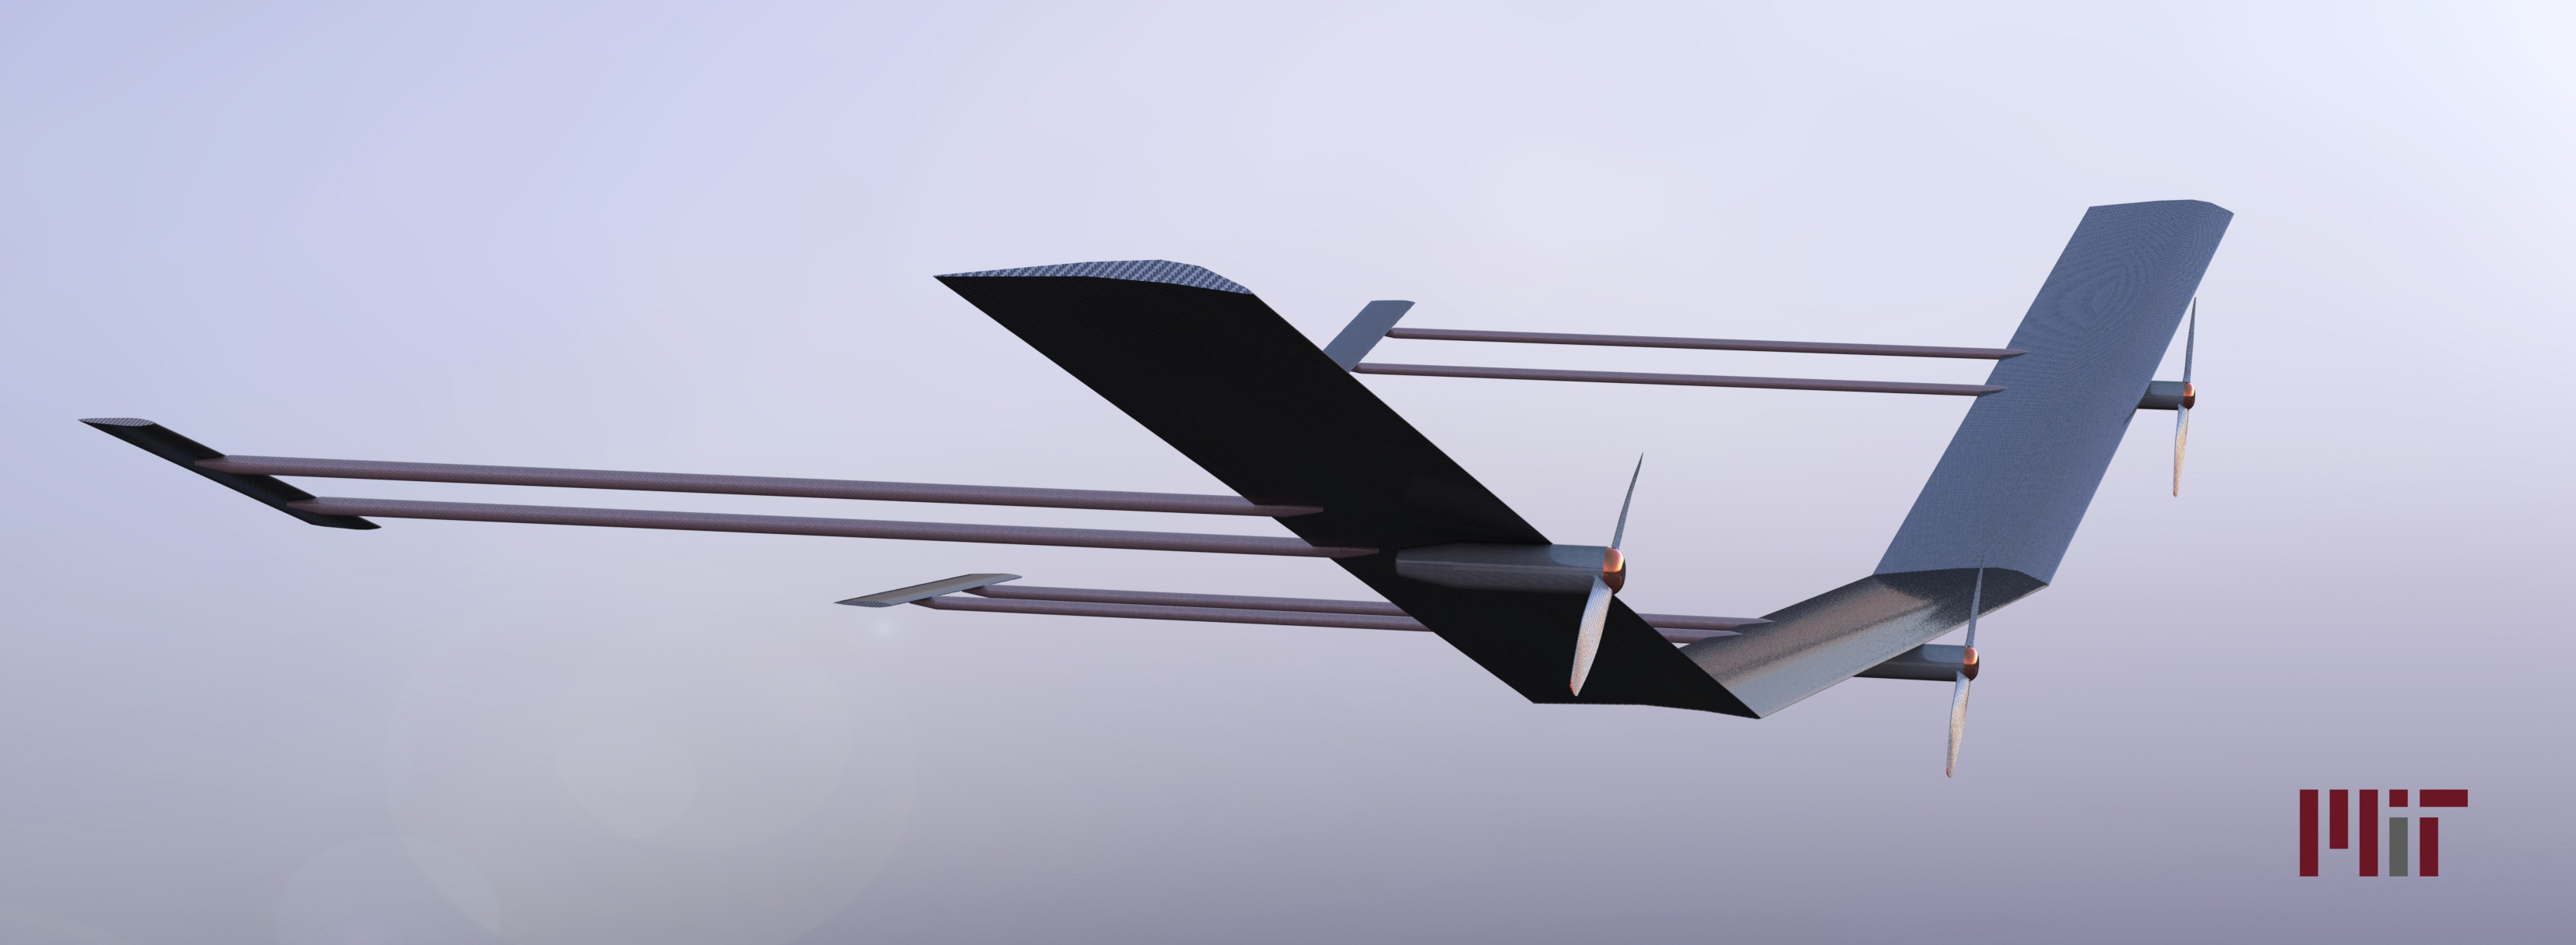
\includegraphics[width=0.95\columnwidth]{../fig/VFA_16.jpg}
	\caption{Rendering of very flexible aircraft model}
	\label{fig:vfa}
\end{figure}

The VFA model consists of three rigid lifting sections which are hinged together such that the aircraft is able to bend at the joints of the three sections. In this example, we consider the longitudinal dynamics of this aircraft. The longitudinal dynamics of this nonlinear model are defined by the state vector
\begin{equation}
x_{\text{vfa}} = \begin{bmatrix}
V \\
\alpha \\
h \\
\theta \\
q\\
\eta\\
\dot{\eta}
\end{bmatrix} =
\begin{bmatrix}
	 $Airspeed (ft/s)$\\ $Angle of attack (rad)$\\ $Altitude (ft)$\\ $Pitch angle (rad)$\\ $Pitch rate (rad/s)$\\ $Dihedral (rad)$\\ $Dihedral rate (rad/s)$
\end{bmatrix}
\end{equation}

We linearize and trim the aircraft in straight and level flight using the inputs
\begin{equation}
	u_{\text{vfa}} = \begin{bmatrix}
\delta_{th} \\
\delta_{a,c} \\
\delta_{a,o} \\
\delta_{e,c} \\
\delta_{e,o} 
\end{bmatrix} = \begin{bmatrix}
		$Thrust (lbf)$\\
		$Center aileron (rad)$\\
		$Outer aileron (rad)$\\
		$Center elevator (rad)$\\
		$Outer elevator (rad)$
	\end{bmatrix}
\end{equation}

For the purposes of this simulation, altitude deviations are assumed to be small, and thus
\begin{equation}
	x_p = \begin{bmatrix}
V & \; \alpha & \; \theta & \; q & \; \eta & \; \dot{\eta}
\end{bmatrix}^T
\end{equation}

The scenario of interest concerns the tracking of commands for the dihedral angle and vertical acceleration, using control inputs $\delta_{a,o}$ and $\delta_{e,c}$ only, so
\begin{equation}
	u_p = \begin{bmatrix}
\delta_{a,o} & \; \delta_{e,c}
\end{bmatrix}^T
\end{equation}

Control of the dihedral angle is desired as a large dihedral angle is inefficient for lift generation (and is open-loop unstable), while a small dihedral angle will require more control effort to hold, increasing drag and power requirements while also potentially twisting the aircraft. 

The measurements available for control design are the pitch rate, dihedral angle, and vertical acceleration, leading to plant output matrices
\begin{equation}
\begin{aligned}
y_p =& \, \Big[\; q \; \Big] \;= \Big[\: \text{Pitch rate (rad/s)} \:\Big] \\
z_p =& \begin{bmatrix}
\eta \\
A_z
\end{bmatrix} =\begin{bmatrix}
	$Dihedral angle (rad)$\\
	$Vertical acceleration (ft/s)$
\end{bmatrix}		
\end{aligned}
\end{equation}
and the augmented plant output matrix 
\begin{equation}
y = \begin{bmatrix}
	q \\ \int{z_p - z_{cmd}}
\end{bmatrix}
\end{equation}

The vehicle is trimmed at an airspeed of $68$ ft/s, altitude of $40,000$ ft, $2.8^\circ$ angle of attack and pitch angle, and dihedral angles ranging from $0$ to $20^\circ$ in $1^\circ$ increments. Figure \ref{fig:trim-poles} shows the poles of the linearized system for different dihedral angles, and Figure \ref{fig:trim-poles-zoom} shows how the system has unstable poles when trimmed above $11^\circ$ dihedral. Figure \ref{fig:trim-inputs} shows the thrust and control surface deflections for the trimmed VFA model over a range of dihedral angles.

\begin{figure}[htbp]
	\centering
	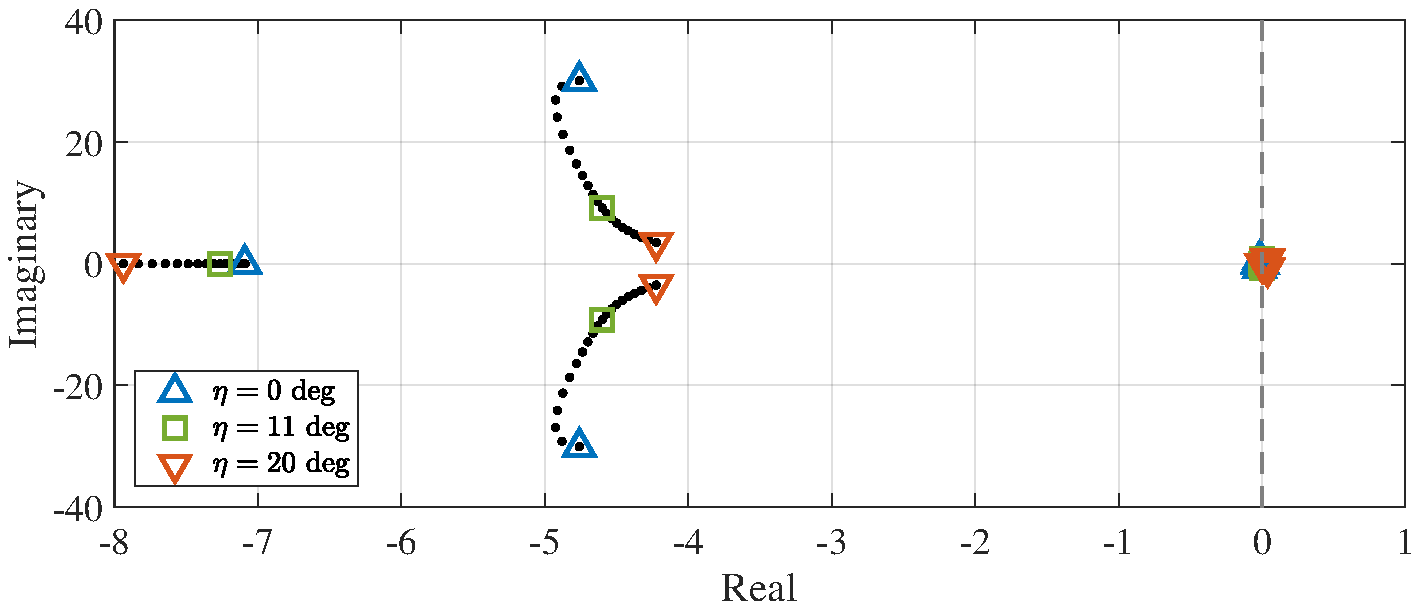
\includegraphics[width=0.95\columnwidth]{../fig/trim-poles-2.pdf}
	\caption{Poles of linearized system for different dihedral angles}
	\label{fig:trim-poles}
\end{figure}

\begin{figure}[htbp]
	\centering
	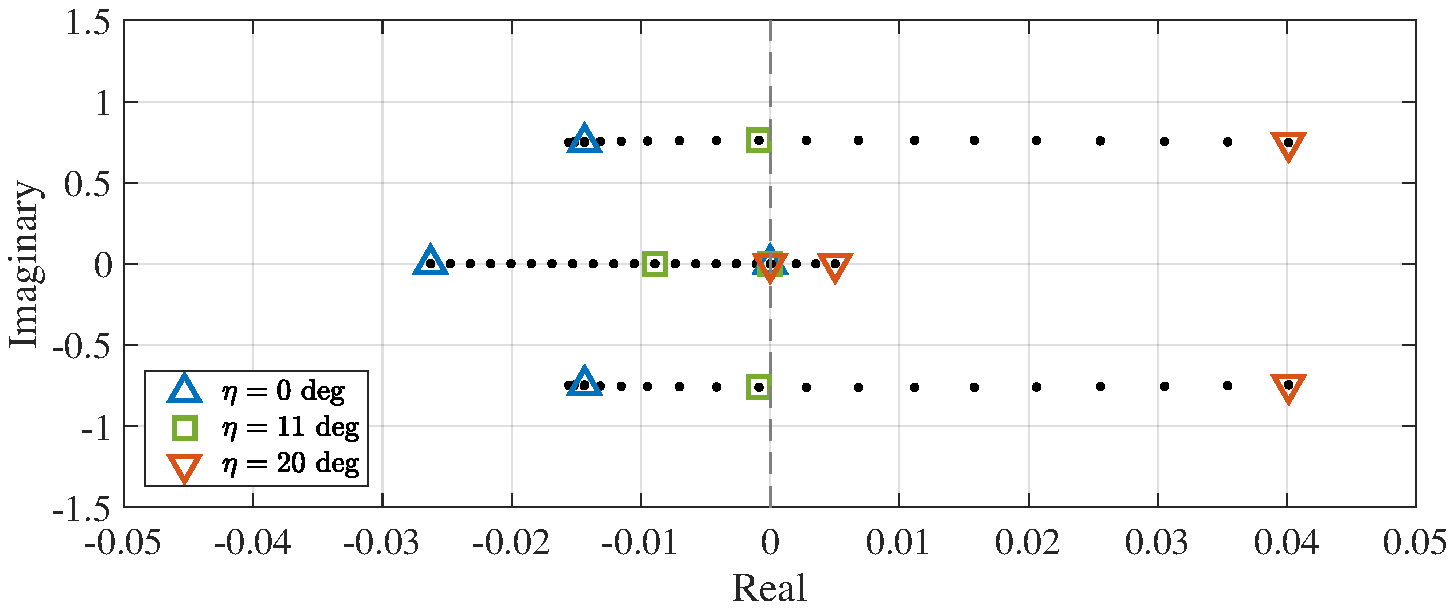
\includegraphics[width=0.95\columnwidth]{../fig/trim-poles-zoom-2.pdf}
	\caption{Dominant poles of linearized system, which move into the right-half complex plane when $\eta > 11^\circ$}
	\label{fig:trim-poles-zoom}
\end{figure}

\begin{figure}[htbp]
	\centering
	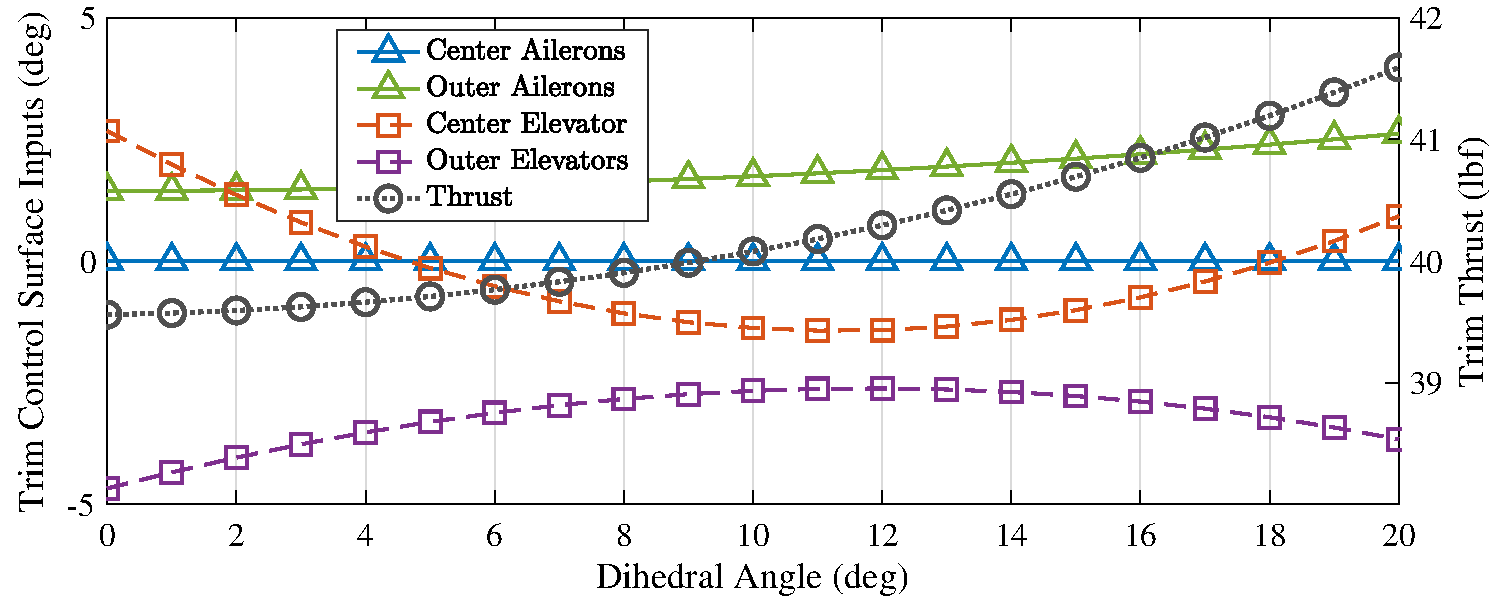
\includegraphics[width=0.95\columnwidth]{../fig/trim-inputs-3.pdf}
	\caption{Inputs to system at different dihedral angles}
	\label{fig:trim-inputs}
\end{figure}

This nonlinear VFA model is augmented with a linear actuator model corresponding to (\ref{eq:first_order_act}) in the nominal case and (\ref{eq:second_order_act}) in the presence of anomalous dynamics. The vehicle simulation with first-order actuators (\ref{eq:first_order_act}) uses time constants $\tau = 2 s$ and $\tau = 1 s$ in the control model and actual plant, respectively, corresponding to
\begin{equation}
D_1 = 2 I_2, \quad \Theta_1 = -1.5 I_2
\end{equation}
where $\Theta_1$ is unknown for control design. Simulation of the anomalous dynamics (\ref{eq:second_order_act}) uses second-order actuators with cutoff frequency $\omega_c = 2$ rad/s and damping ratio $\zeta = 0.7$, and $\omega_c = 1$ rad/s and $\zeta = 0.8$ in the control model and actual plant, respectively, corresponding to
\begin{equation}
\begin{bmatrix}
	D_1 \\ D_2
\end{bmatrix} = \begin{bmatrix}
	4 I_2 \\ 2.8 I_2
\end{bmatrix}, \quad \begin{bmatrix}
	\Theta_1 \\ \Theta_2 
\end{bmatrix} = \begin{bmatrix}
	-3.75 I_2 \\ -2 I_2
\end{bmatrix}
\end{equation}
where $\Theta_1$ and $\Theta_2$ are unknown for control design. In all the following numerical simulations, the uncertainty added to the control model for simulation is
\begin{equation}
\begin{gathered}
\Theta_{p}^{T}=\begin{bmatrix}
0.6 & -4.52 & \; 0 & \hfill 0.05 & \hfill 0.41 & \hfill 1.47\\
0.1 & \hfill 1.83 & \; 0 & -0.02 & -0.35 & -0.59
\end{bmatrix}\\ \Lambda = 0.2 I_2 \end{gathered}
\end{equation}


%\subsection{Shared Control}
%A particular limitation of adaptive control -- and any model-based control design -- is that guarantees on stability margins and command tracking performance may not withstand the presence of unmodeled dynamics. There are many reasons where dynamics (which are either not present or ignored due to their time constants relative to controller bandwidth) that are not accommodated in control design may become more severe due to faults or dynamical anomalies during operation. For many autonomous systems, when an anomaly occurs, the solution is to transfer control to a human pilot (onboard or remote) to attempt to control the vehicle manually. This transfer to manual control, and the unfamiliarity of the anomalous dynamics to the pilot, may lead to loss of control of the vehicle. We suggest the use of a shared decision-making and control framework in which a human operator is responsible for detecting a dynamical anomaly but not for taking over control of the aircraft, first proposed in \cite{thomsen2018shared}. In the following simulation, we demonstrate an example of how this is possible.

\subsection{Numerical Simulations}
Numerical simulations have been carried out for the longitudinal and dihedral dynamics of the HALE VFA described in the preceding sections. 

We first simulate nominal UAV operation (first-order actuators) to demonstrate the effectiveness of the adaptive autopilot during normal operation. We simulate three cases:
\begin{description}
	\item[Nom-1] Baseline RSLQR without uncertainty in control model
	\item[Nom-2] Baseline RSLQR with uncertainty in control model ($\Theta_p$, $\Lambda_p$, and $\Theta_1$)
	\item[Nom-3] Baseline RSLQR + MRAC with uncertainty in control model ($\Theta_p$, $\Lambda_p$, and $\Theta_1$)
\end{description}

These simulations, presented in Figs. \ref{fig:nom1}, \ref{fig:nom2}, and \ref{fig:nom3} respectively, show how the MRAC controller with output feedback described in (\ref{eq:rd2-b1a})--(\ref{eq:rd2-adaptation}) is able to recover the desired closed-loop performance in the presence of uncertainty of plant and actuator parameters. The closed-loop system with the baseline RSLQR controller does not lose stability in the presence of uncertainty (Fig. \ref{fig:nom2}), however the tracking performance suffers, especially for vertical acceleration tracking.

\begin{figure}[htbp]
	\centering
	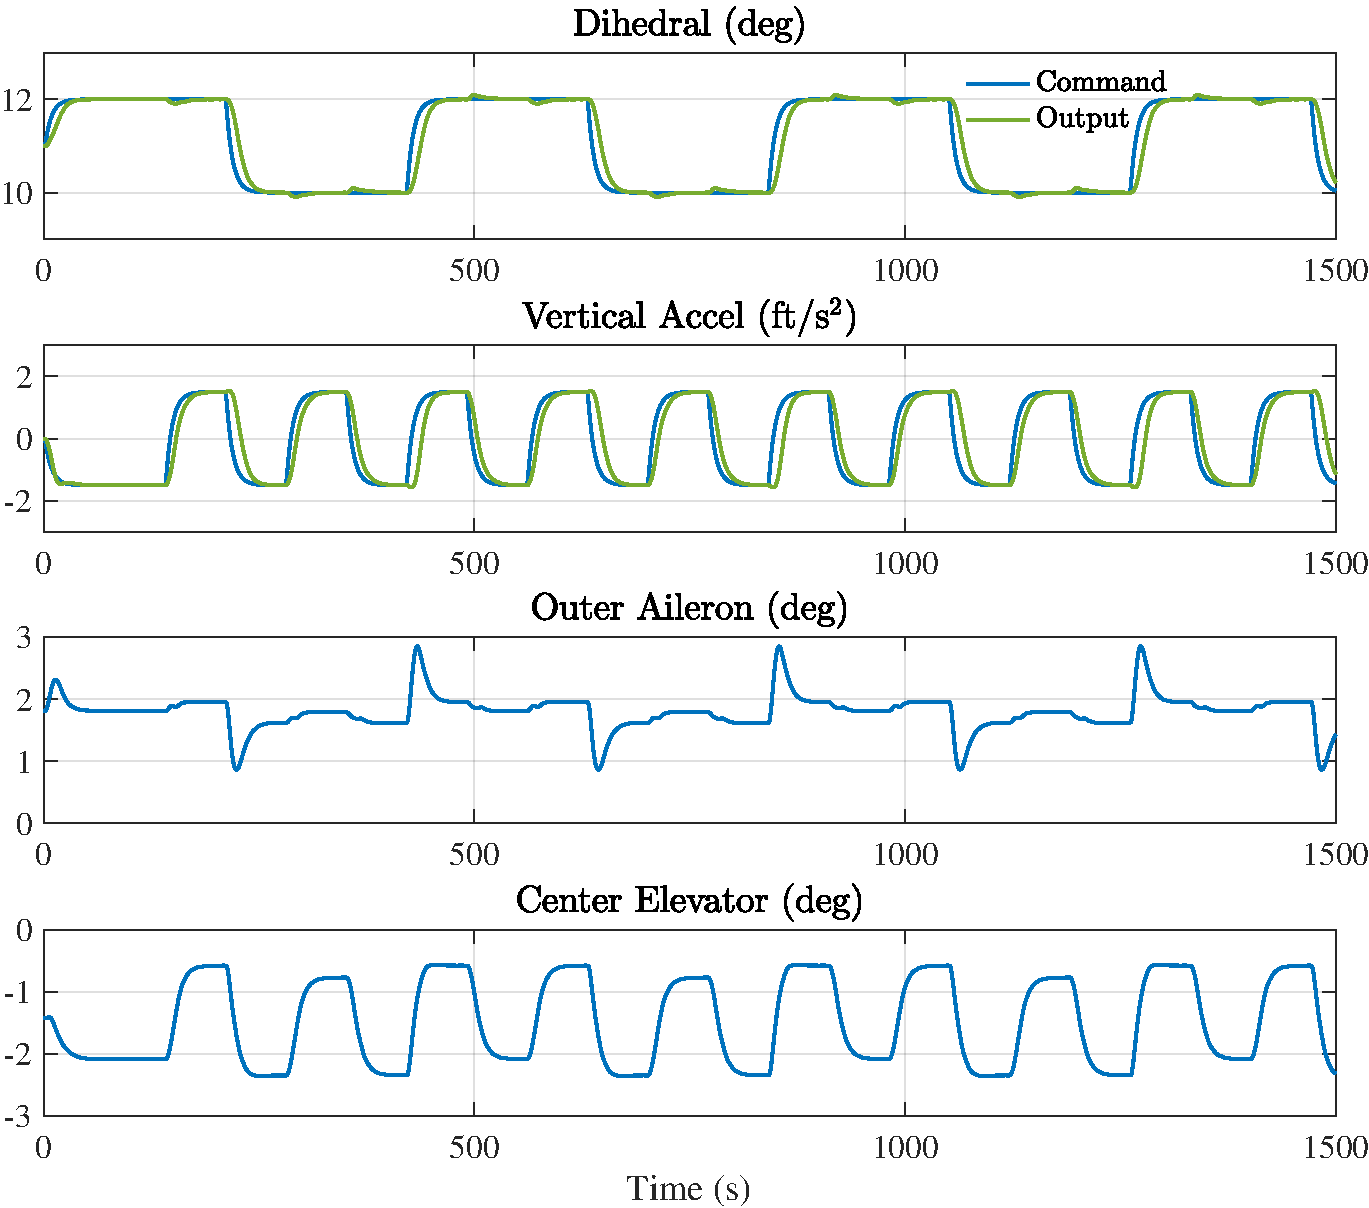
\includegraphics[width=\columnwidth]{../fig/nom1.pdf}
	\caption{Nom-1 simulation: RSLQR with no uncertainty in the control model}
	\label{fig:nom1}
\end{figure}

\begin{figure}[htbp]
	\centering
	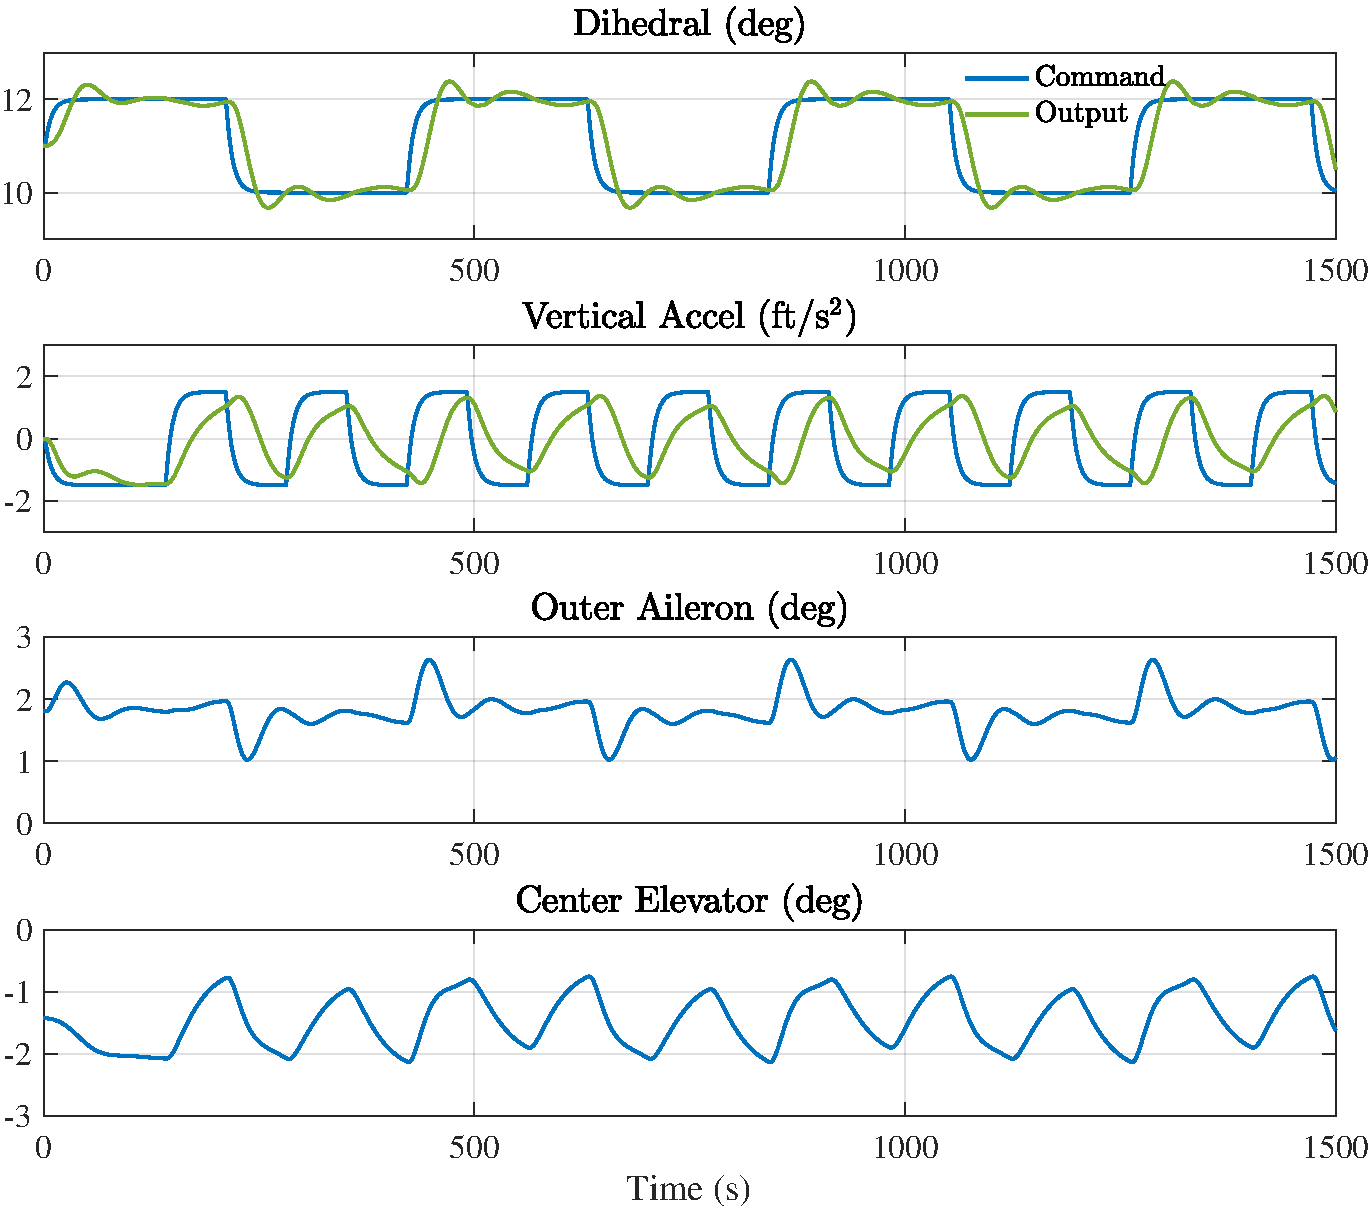
\includegraphics[width=\columnwidth]{../fig/nom2.pdf}
	\caption{Nom-2 simulation: RSLQR with uncertainties $\Theta_p$, $\Lambda_p$, and $\Theta_1$}
	\label{fig:nom2}
\end{figure}

\begin{figure}[htbp]
	\centering
	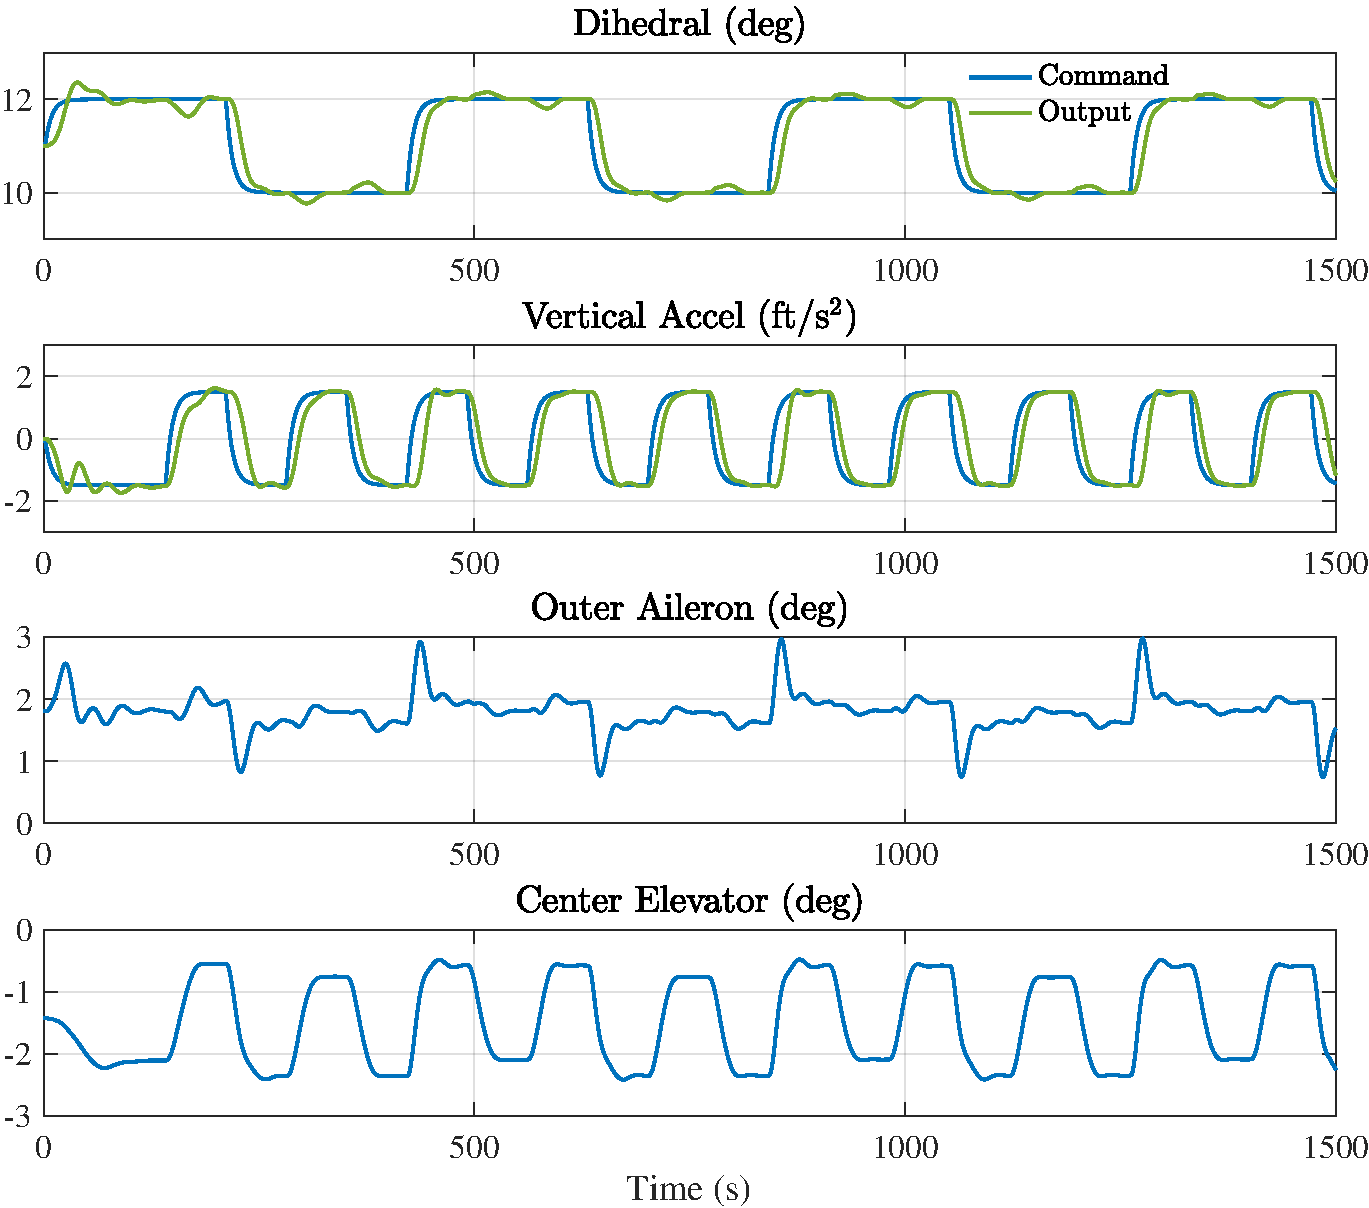
\includegraphics[width=\columnwidth]{../fig/nom3.pdf}
	\caption{Nom-3 simulation: RSLQR + MRAC with uncertainties $\Theta_p$, $\Lambda_p$, and $\Theta_1$}
	\label{fig:nom3}
\end{figure}

We now simulate several responses to the introduction of a severe anomaly to demonstrate the effectiveness of the shared control response described in Section \ref{sec:shared_ctrl}, and compare its performance to alternative responses. The severe anomaly which we introduce is the change in actuator dynamics from the uncertain first-order dynamics (\ref{eq:first_order_act}) to the uncertain second-order dynamics (\ref{eq:second_order_act}). The three anomaly responses we consider are
\begin{description}
	\item[AR-1 (Passive/Autonomous)] The RSLQR+MRAC autopilot continues without any intervention from remote human supervisor
	\item[AR-2 (Manual Control)] The human operator takes over manual control of the affected vehicle
	\item[AR-3 (Shared Control)] Responsibilities are shared between the human pilot and autopilot to safely recover from introduction of unmodeled dynamics
\end{description}

In all the following simulations, the vehicle operates in nominal operation with the adaptive controller and baseline RSLQR control design for $0 \leq t < 600 s$. At $t = 600 s$, the anomaly is introduced suddenly, corresponding to a failure which causes the vehicle's actuators to change from first-order to second-order. Figs. \ref{fig:ar1}--\ref{fig:ar1-err} show the result of a passive response (AR-1) in which the human operator ignores controller performance degradation and allows the adaptive controller to continue in the presence of severe unmodeled dynamics. Most notably, the closed-loop system loses stability leading to large oscillations in vehicle state and eventual structural failure of the VFA after $t = 960s$, or 6 minutes after the anomaly introduction. Also notable are the rapid increase in magnitude of the adaptive parameters and the magnitudes of both tracking and measurement output error signals after the introduction of anomalous dynamics.

\begin{figure}[htbp]
	\centering
	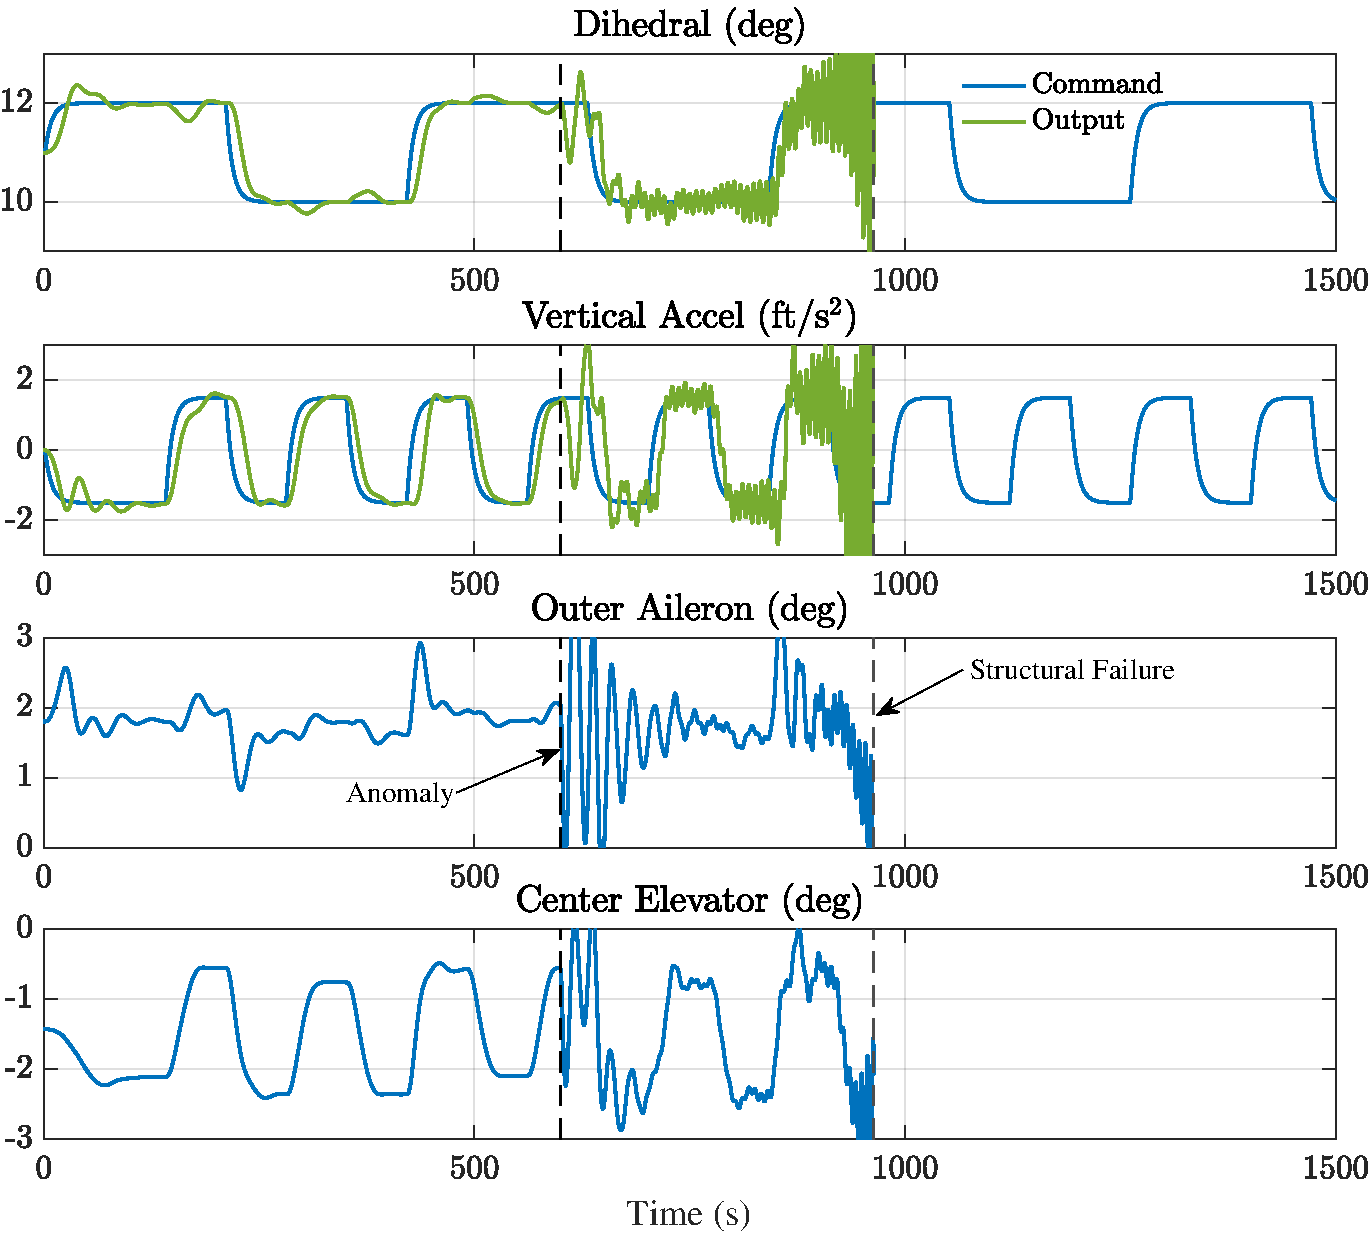
\includegraphics[width=\columnwidth]{../fig/ar1.pdf}
	\caption{AR-1 simulation: passive response to dynamical anomaly results in structural failure after 6 minutes}
	\label{fig:ar1}
\end{figure}

\begin{figure}[htbp]
	\centering
	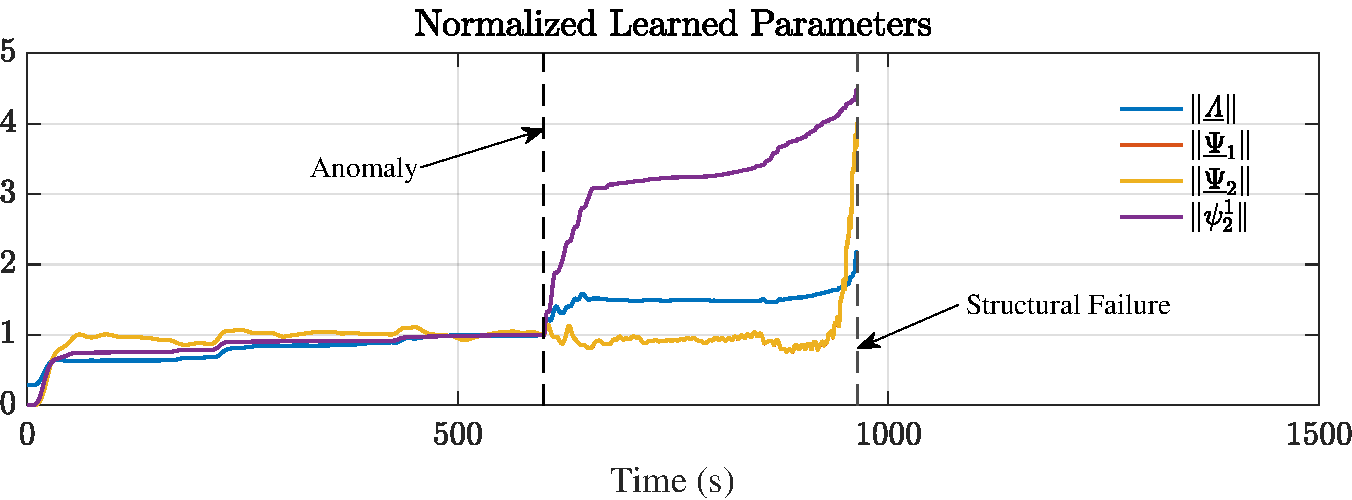
\includegraphics[width=\columnwidth]{../fig/ar1-params.pdf}
	\caption{AR-1 simulation: adaptive parameters diverge as controller struggles to adapt to unmodeled dynamics}
	\label{fig:ar1-params}
\end{figure}

\begin{figure}[htbp]
	\centering
	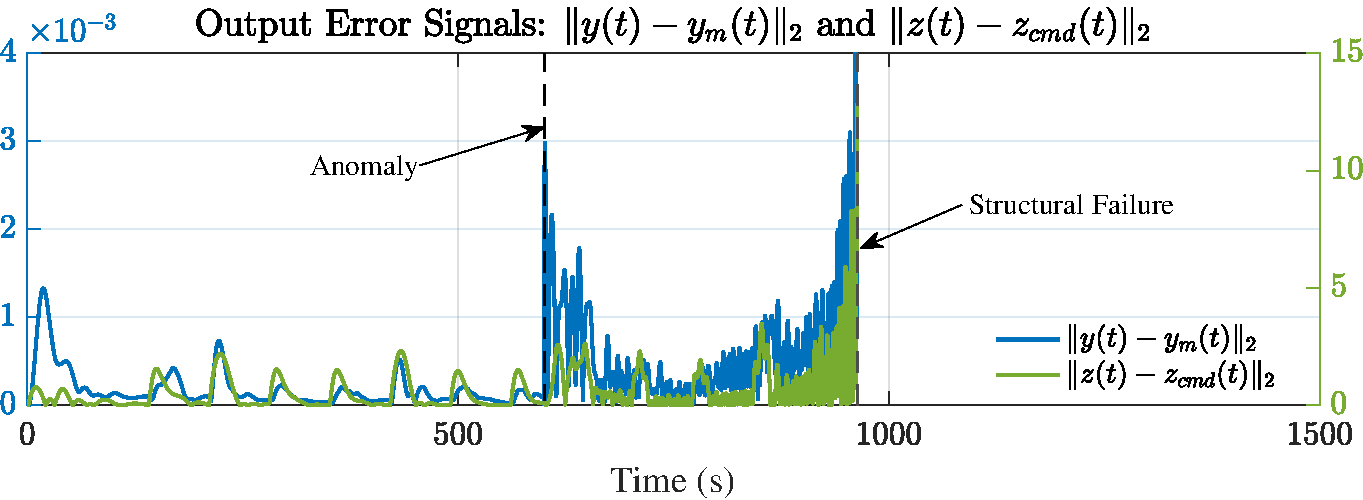
\includegraphics[width=\columnwidth]{../fig/ar1-err.pdf}
	\caption{AR-1 simulation: model-following output error and command tracking error grow due to anomalous dynamics}
	\label{fig:ar1-err}
\end{figure}

Numerical simulations of the AR-2 response (purely manual control) are not carried out, as they are not deterministic and require high-fidelity human-in-the-loop experiments to characterize. The limitations of such a response -- in which the human operator's role changes suddenly from ``on-the-loop'' to ``in-the-loop'' with unfamiliar dynamics -- are discussed in the earlier sections of this paper.

The AR-3 (shared control) anomaly response simulation is shown in Figs. \ref{fig:ar3-sim}--\ref{fig:ar3-err}. After the anomaly is introduced at $t = 600 s$, the ``nominal'' controller attempts to control the system which has severe unmodeled dynamics until $t = 800 s$, which is the culmination of the human operator's action. In the shared control framework, the human operator notices the anomalous closed-loop control behavior, and via an interface switches the controller to a higher relative degree model in the control design. For $t \geq 800 s$, the vehicle remains under autonomous control and is able to recover stability and tracking performance. For comparison, the time of structural failure in the passive anomaly response is plotted as a line at $t = 960 s$.

\begin{figure}[htbp]
	\centering
	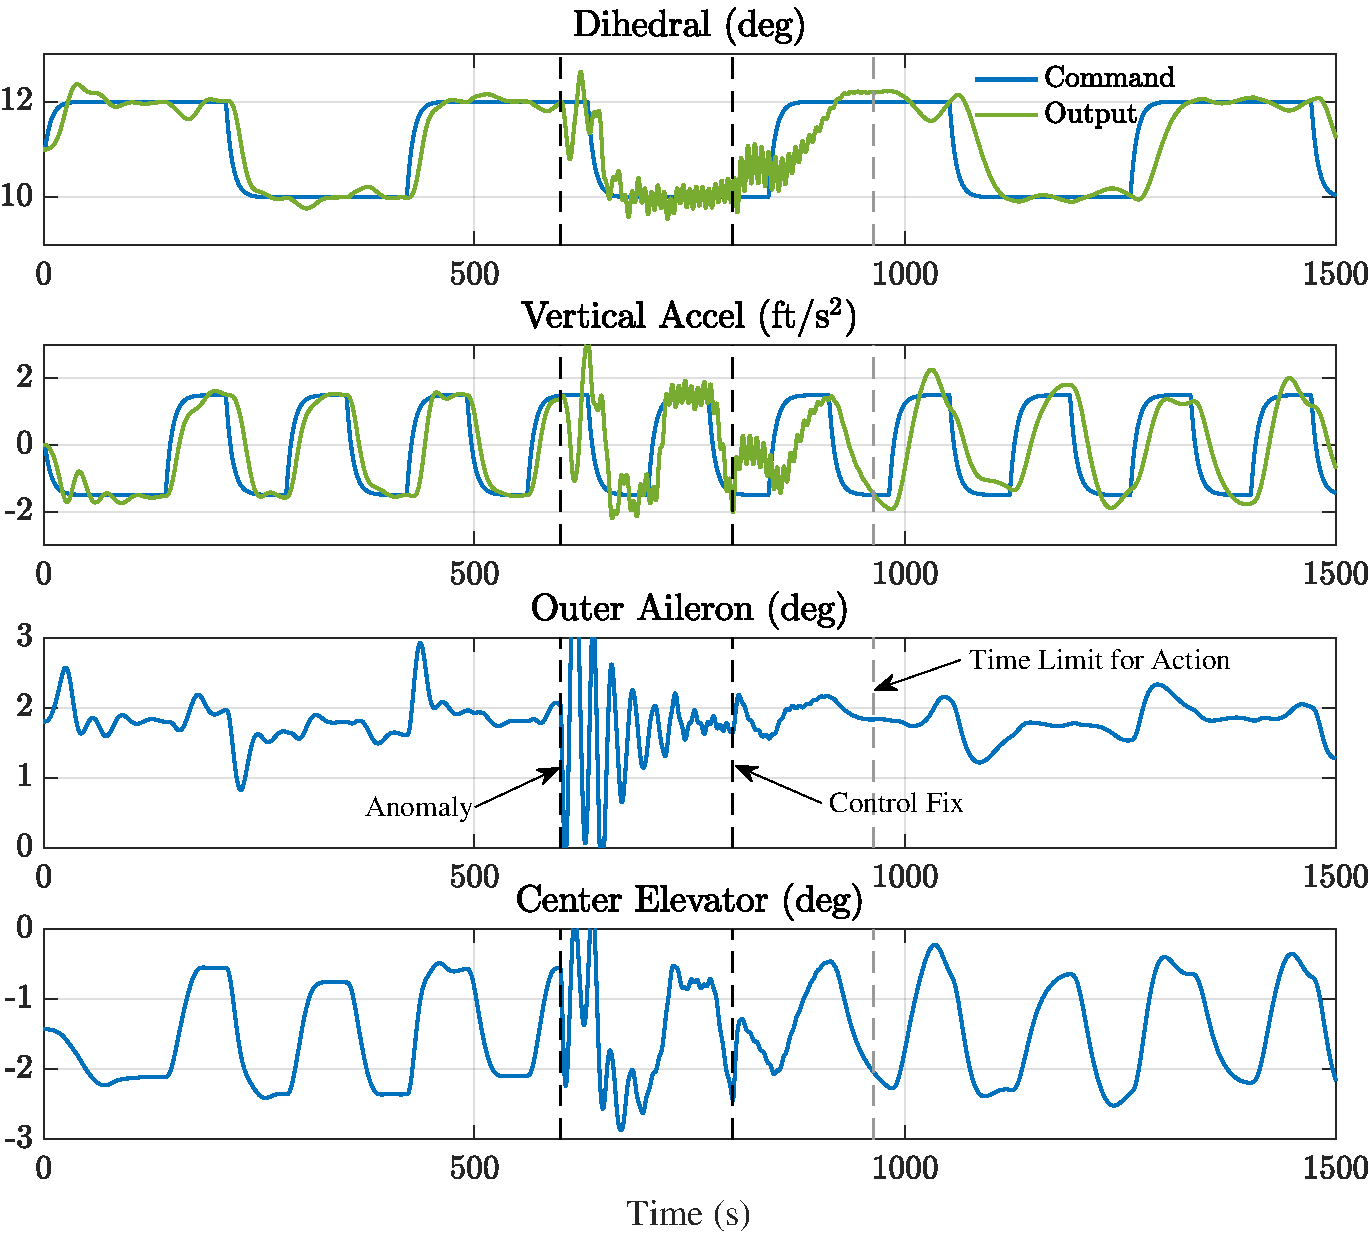
\includegraphics[width=\columnwidth]{../fig/ar3.pdf}
	\caption{AR-3 simulation: shared response to the dynamical anomaly results in recovery of vehicle performance}
	\label{fig:ar3-sim}
\end{figure}

\begin{figure}[htbp]
	\centering
	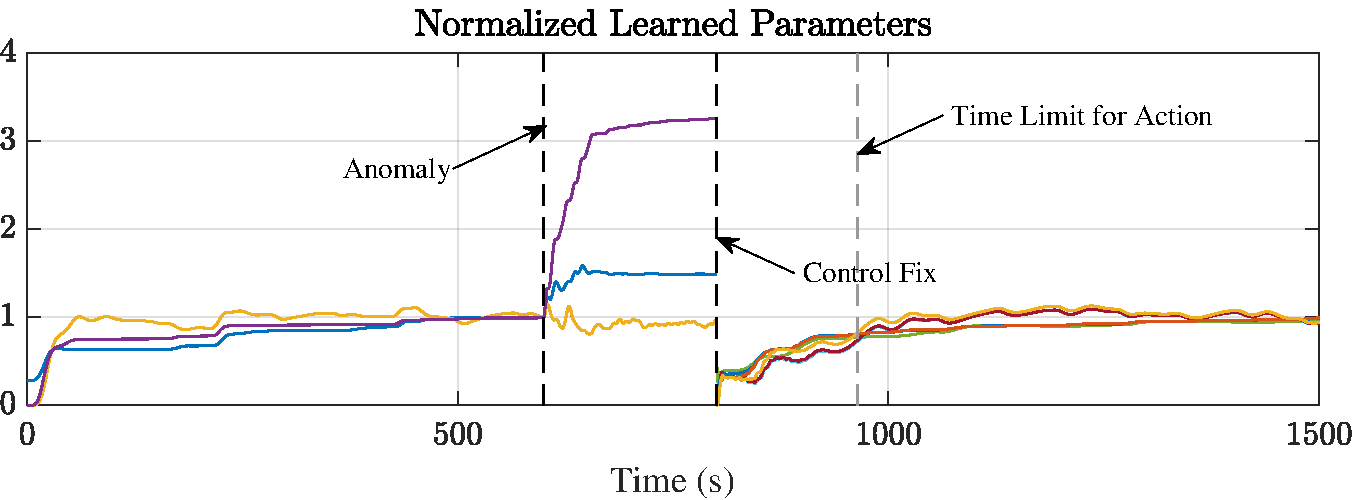
\includegraphics[width=\columnwidth]{../fig/ar3-params.pdf}
	\caption{AR-3 simulation: the change in control model at $t = 800 s$ stops the divergence of adaptive parameters}
	\label{fig:ar3-params}
\end{figure}

\begin{figure}[htbp]
	\centering
	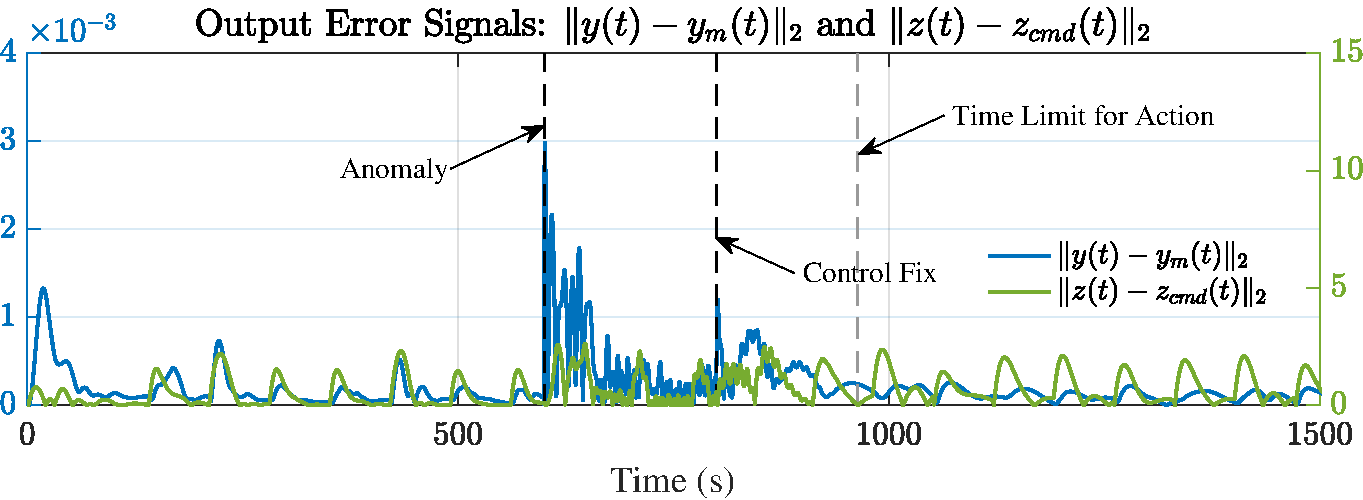
\includegraphics[width=\columnwidth]{../fig/ar3-err.pdf}
	\caption{AR-3 simulation: the change in control model at $t = 800 s$ stops the error growth seen after the anomaly}
	\label{fig:ar3-err}
\end{figure}

\bibliography{thomsen-cphs-2018-bib}
\end{document}
